\chapter{Methodology}

The most important components of this study are the data sets being constructed for each of the bird species. Before talking about the appended climate data and the bird species themselves, it is worthwhile to first go over the given attributes of the Project FeederWatch (PFW) data set. These initial attributes largely determined the format and characteristics of the climate data.

\section{Given Attributes of the Project FeederWatch Data}

There are a total of 18 different attributes for each tuple in the original FeederWatch data. The complete list of these features is below, and of course not all of them were applicable to this project. These descriptions were obtained through the guidelines provided by PFW. The actual guideline document can be found in Appendix B.

\begin{itemize}

  \item Latitude: The latitude value of the observation location in decimals. No information was given about how this measurement was done or how accurate is it to the actual location. This is relevant to the project as this is used to establish a city location for a given observation. This city location is later used to fetch the climate data.
  
  \item Longitude: The longitude value of the observation location in decimals. No information was given about how this measurement was done or how accurate is it to the actual location. Similar to Latitude, this was relevant to the project for establishing a city location.
  
  \item ID: This is the identification number of the participant in Project FeederWatch. This is a unique Cornell Lab of Ornithology identification number and it is not available to the public. This value served no purpose in this study.
  
  \item StatProv: This is the U.S. state or Canadian province of the observation location. We are only focused on the continental United States and this state information is vital. It is used to establish the city for a given observation.
  
  \item Entry Technique: These are the various methods of the identifying the latitude and longitude values for a given observation. This is not relevant to the focus of this study and thus not considered.
  
  \item FW Year: This is the FeederWatch season. The seasons run from November to April, thus only covering the winter season. Example, 'PFW--1992' indicates the season running from November 1991 to April 1992. These values were ignored for this project as the \textbf{Year} attribute below provided the year information for each PFW observation.

  \item Year: This is the year of the first day of the two-day count observation. This was relevant to this project as this was used to query the dated climate data.
  
  \item Month: The month of the first day of the two-day count observation, used to fetch the appropriate climate data. See Year.
  
  \item Day: The day of the observation. This is for the first day of the two-day count. This value was used to fetch the correct climate data. See Month and Year.
  
  \item NHalfDays: This is the number of the half days of the observation during the two-day count period and is used as a measure of observer effort. The half days range from 1 to 4. This quantification was taken into account in the data models used for analysis. See the Data Analysis section.  
  
  \item Effort Hrs Atleast: Another measure of the observer's effort. This is a measure of how many hours the participant invested making the observations. This ranged from less than 1 hour to greater than 8 hours. This quantification was taken into account in the data models used for analysis. See the Data Analysis section.   
  
  \item BirdSpp: This is the name of the species seen at the feeder for a given observation. This is a crucial feature for this project. One of the main questions of this study deals with different sized bird species. The bird species attribute was used to filter out data only pertaining to the species of focus, as due to time constraints only a portion of the PFW data could be processed. These bird species were decided upon consultation with our field expert Professor Francis. More about this is covered in the Bird Species Selection section.
  
  \item NSeen: The number of individuals seen, this is the maximum number of the species in view at a single time over the two-day observation period. Another crucial attribute for the project. This data is relevant because it is a quantification of how many individuals of the bird species are using the bird feeders as a food source.
  
  \item Valid: This is a flag used to preserve data quality. In regards to this project, the data has already been filtered to only include valid and reviewed data. These data values are not relevant to this study.
  
  \item Reviewed: This is a flag used to preserve data quality. Again within the context of this project, the data is already reviewed. Thus, these values are not used. See Valid above.
  
  \item Loc ID: This is the unique identifier for the location of the observation. Note that participants, see ID above, can have multiple count locations or Loc ID's. This data is not relevant. 
  
  \item Sub ID: This is the submission identifier and it uniquely identifies the entire checklist submitted by a participant from the count period. Note, if the species observations are all on the same checklist, then they have the same Sub ID. This is not relevant for the project.
  
  \item Obs ID: This is the observation identifier and it uniquely identifies a single observation. All species reported on a single checklist receive different observation identifiers. This data is not relevant for this study.

\end{itemize}

To summarize, there are many attributes to the PFW data set, but only a handful are useful for this project. The latitude, longitude and states data are all key to this project as they are used to establish a U.S. city location for which climate data can be collected. Additionally, the year, month and day values are important as they ensure the climate data is correctly dated. As a reminder this a winter season study, and the season ranges from November to April. Nseen is the main quantification of the abundance of a bird species at a given feeder location and is used to quantify how many individuals are using the feeders. Note again, the count period for the number seen is 2 days. Lastly, there is bird species, and this is one of the most important attributes. It is covered in detail in the Bird Species Selection section.

The hours of effort, location id and number of half days are all factors taken into account for the data analysis and is covered in the later sections. These attributes are only relevant for results and conclusions portions of the project. The rest of the attributes included with the Project FeederWatch data are simply ignored as they are not relevant to the questions being tackled.  

\section{Bird Species Selection}

When selecting bird species for this study, 3 main factors became the driving force. First, the bird species must be non-migratory during the winter season. This filtering criteria ensures that the bird species for this study remain in their respective regions and actually experience the colder climate of winter. The only exception to this requirement is the Evening Grosbeak. However, the species was chosen for this study because of the previous work done on it in regards to the population decline at the feeders. 

Second, the bird species must be well represented in the PFW data set. Our criteria being that the bird species must at least have a few hundred observations. This will ensure that there is enough data to develop models for after the filtering and clean up steps. The exact details of these data processing steps are covered in the next few sections. 

The third factor in the bird selection process was the body mass of the species. As a reminder the focus of the project revolves around how different massed birds react to cooler temperatures, with the main comparison being between smaller species and mid to large species seen at the feeders. Thus, the aim of the final selection was to have about the same number of smaller massed bird species as the mid to larger sized bird species. Our biology expert, Professor Francis, offered valuable consultation in selecting the species and also in ensuring the requirements above were met.

The final set of bird species that was selected is presented in Table 3.1. This table contains all of the bird species that are used for this study. The first criteria of the bird species being well-represented in the original PFW dataset is met as many of the species have tuples numbering in the thousands, with the only exception being Pine Grosbeak. 

However, another issue arises with some species having too many tuples, as there are daily limitations on how much climate data can be collected through WU's API. For example, the number of observations for Mourning Dove is 153,417 and the time required for appending climate data to all of the observations would be in terms of weeks not hours given the limitations. This makes processing all of the observations for the 23 species impractical. For this reason only a maximum of 5,000 observations per each bird species were used for the climate data collection. These 5,000 observations were chosen at random. This allows us to obtain climate data for all of the 23 bird species, while still having enough observations for further data processing and modeling.   

The second goal of including roughly equal numbers of small, mid and large sized bird species is also met as clearly shown by the average body mass measurements in the table. The mean body mass values, in grams, are presented in the column labeled Body Mass of Table 3.1 and these averages were calculated using values from the Cornell Ornithology Lab's website All About Birds and the bird mass handbook by John B. Dunning Jr.~\cite{AllAboutBirds:online, dunning2007crc}. The number of observations for each species in the original PFW dataset is presented in the column labeled PFW Observations. 

The number of the observations per species that were used in the final data models and analysis are presented in the column Filtered Obs. The filtration and data processing methods used to obtain the final tuples in Filtered Obs. are covered in the later sections. 

% Please add the following required packages to your document preamble:
% \usepackage{longtable}
% Note: It may be necessary to compile the document several times to get a multi-page table to line up properly
\begin{longtable}[c]{|l|l|l|l|}
\caption{Bird Species and the number of observations used in this study.}
\label{my-label}\\
\hline
Bird Species              & Body Mass (grams) & PFW Observations & Filtered Obs. \\ \hline
\endhead
%
American Goldenfinch      & 15.5              & 133496           & 4054          \\ \hline
Black-billed Magpie       & 177.5             & 3704             & 3287          \\ \hline
Black-capped Chickadee    & 11.5              & 102562           & 2648          \\ \hline
Blue Jay                  & 85                & 106666           & 1264          \\ \hline
Brown Creeper             & 7.5               & 7457             & 4770          \\ \hline
Chestnut-backed Chickadee & 9.5               & 11992            & 4643          \\ \hline
Chipping Sparrow          & 13.5              & 13004            & 3158          \\ \hline
Common Grackle            & 108               & 25920            & 2720          \\ \hline
Common Redpoll            & 15.5              & 4545             & 3615          \\ \hline
Dark-eyed Junco           & 24                & 159161           & 5000          \\ \hline
Downy Woodpecker          & 24.5              & 137064           & 4699          \\ \hline
European Starling         & 78                & 57676            & 4408          \\ \hline
Evening Grosbeak          & 63.5              & 1595             & 1206          \\ \hline
Hairy Woodpecker          & 67.5              & 50665            & 4691          \\ \hline
Mountain Chickadee        & 11                & 5140             & 2995          \\ \hline
Mourning Dove             & 121               & 153417           & 2876          \\ \hline
Northern Mockingbird      & 51.5              & 26507            & 4792          \\ \hline
Northern Cardinal         & 45                & 147259           & 2118          \\ \hline
Pine Grosbeak             & 56.4              & 250              & 231           \\ \hline
Pine Siskin               & 15                & 27250            & 2738          \\ \hline
Red-bellied Woodpecker    & 73.5              & 91767            & 4685          \\ \hline
Tufted Titmouse           & 22                & 113012           & 4811          \\ \hline
White-throated Sparrow    & 27                & 61422            & 4517          \\ \hline
All Species               & NA                & 1441531          & 79926         \\ \hline
\end{longtable}


\section{Given Attributes of Weather Underground Data}

There are over a hundred climate attributes provided by Weather Underground, ranging from the standard average temperature values to the very specific measurements of cooling days since the first day of the year~\cite{WUAPI:online}. There are far too many attributes to list and discuss individually, instead listed below are the climate measurements that were deemed important and relevant according to our domain expert Professor Francis. From this initial set of attributes the final 6 were eventually chosen for the actual study.

An important note, for the historical climate data, Weather Underground has 2 categories for each of the climate features, observations and daily summaries~\cite{WUAPI:online}. Observations are all of the direct climate measurements for the day. For example, the hourly temperature values, for which there will 24 measurements. While the daily summary is, as the name implies, a single summary value for the day. For example, the mean temperature calculation for the day or the average wind speed for the day, both are single values for the day. For the scope of this study, only daily summary values are useful as it is a single average measurement for the day, which can then be appended to the PFW observation with same day. The observations are ignored as there may be multiple observation values for one day. The listed climate features below are all from the daily summary category.

\begin{itemize}

  \item date: This is the date of the observations. This is very relevant to the study as this ensures that the correctly dated climate values are collected for the PFW data.
  
  \item percipi: Precipitation in inches of rain. This feature is also relevant to this project. An important note, WU provides the precipitation measurements both in inches and millimeters, but only the inches value was collected. This is because the data can be later converted if necessary.
  
  \item snowfalli: Snowfall in inches of snow. Though this is an important climatic factor, it is not going to be focused on in this project.
  
  \item humidity: Humidity represented as a percentage. Again, this may be important for other studies, but for this study these values are ignored.
  
  \item maxtempi: Maximum temperature value for the day in Fahrenheit. This is relevant to this project as one of the main questions is to analyze bird species abundance around bird feeders in regards to temperature. Note, Weather Underground does provide the temperature measurements in Celsius, but only the Fahrenheit values were collected. The idea being that the values can be easily converted in the future if required.  
  
  \item mintempi: Minimum temperature value for the day in Fahrenheit. This is relevant to this study, see maxtempi.
  
  \item meantempi: Mean temperature value for the day in Fahrenheit. This is relevant to this project, see maxtempi.
  
  \item meanwspdi: Mean windspeed for the day in miles per hour. This is relevant to this study as one of the main questions is to determine whether wind speed has an affect on bird abundance at the bird feeders. Note, Weather Underground does provide the speed in kilometers per hour, but only the miles per hour values were collected. The values can be converted and appended later if required.
  
  \item minwspdi: Minimum wind speed for the day in miles per hour. This is not relevant to this study as the mean wind speed for the day is more useful for determining the wind conditions throughout the day, see meanwspdi.
  
  \item maxwspdi: Maximum wind speed for the day in miles per hour. This is not relevant to this study as the mean wind speed for the day is more useful for determining the wind conditions throughout the day, see meanspdi.
  
\end{itemize}

To summarize, of the subset of the climate features presented above the final group of relevant attributes are as follows: date, precipi, mintempi, maxtempi, meantempi, and meanwspdi. Eventually only the mean temperature was deemed relevant for the actual study in terms of the temperature measurements. The minimum and max temperature values were ignored for the analysis. The details of this will be covered in the Preprocessing for Data Models section. The date is vital to ensure the climate measurements are from the same date as the PFW observation. The precipi values were also deemed relevant for this project. Finally, only the mean wind speed values (meanwspdi) were used in the study, while the max and min wind speed values were ignored. Further information about the reasoning behind these selections is in the next section.


\section{Script Implementation for City Attribute}

Before the Weather Underground's API can be utilized, the PFW data needs additional location details besides just latitude, longitude and state values of the bird feeders. The majority of the population of United States lives within major city areas~\cite{sutton1997comparison}, as a result much of the data from PFW and WU are from these densely populated urban areas. The challenge now is to filter out all of the bird feeders that are located too far away from a major city.

The pseudo code for the following steps is presented in Algorithm 1. The first step is to load the original PFW data into a data frame which can then be logically manipulated. Next, there is the loop that iterates through each row of the data frame. For each row, or observation, the latitude, longitude and state values become the parameters for the method getNearestCity(). This method is then called and the return value is stored in the variable city.

The getNearestCity() method is key to this procedure as this determines whether the bird feeder location is close enough to a city. This function contains the top 1,000 U.S. cities and their latitude, longitude and state values in a key value pair data structure. With the given bird feeder location parameters, the distances between the feeder and the nearest major cities of the state are calculated. 

The city with the minimum distance is then returned, as this will provide the nearest location for a Weather Underground weather station. If the bird feeder is more than 40 kilometers away from the city, then that city is not considered and ignored. If no suitable major city is found, then getNearestCity() will return NULL and that row is deleted from the data frame. Figure 3.1 is a generalized visual representation of the city selection process. 

The last step simply involves converting the data frame to a CSV file and exporting it with the correct file name. At this stage, all of the PFW observations now have a city attribute, for which climate data can acquired through Weather Underground. The actual implementation, in the Python programming language, of Algorithm 1 is presented in Appendix C.   

\begin{figure}[h]
\centering
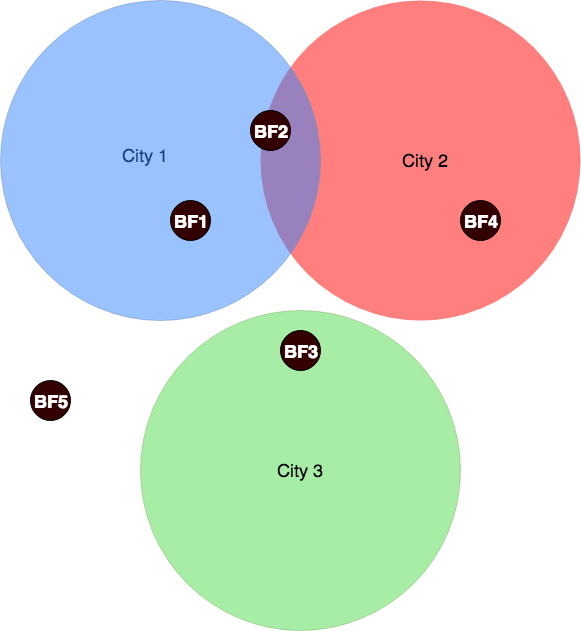
\includegraphics[width=0.5\textwidth]{figures/BFandCities.png}
\caption{This figure illustrates how Algorithm 1 selects a city for a given bird feeder of PFW. The the black circles labeled with BF represents the location of a bird feeder (BF). The colored circles represent a distance radius of 40 kilometers from the city center. For example, the green circle represents distances that are within 40 kilometers from the center of City 3. Given the situation above, BF1 and BF2 would be assigned City 1. Note, even though BF2 is in the range for City 2, it is closer to City 1 and it is picked by the algorithm. BF3 would be assigned City 3 and BF4 would be assigned City 2. Lastly, BF5 is not within 40 kilometers from any major city so all observations with BF5 will be deleted from the final data set as the city is needed for acquiring the climate data. This will be covered in detail in the next section.}
\end{figure}

\begin{algorithm}[H]
\DontPrintSemicolon
\SetKwInOut{Input}{Input}\SetKwInOut{Output}{Output}
\Input{Original Project FeederWatch Data}
\Output{Project FeederWatch Data with cities appended.}
 
$dataFrame\leftarrow "PFWData.csv"$    \;

dataFrame.addColumns("city")
 
\ForEach{Row r in dataFrame}{
	
    \tcc{getNearestCity method returns the city which is at most 40km away from the lat/long coordinates. Returns NULL if no city in the state is found.}
    $city\leftarrow getNearestCity(r.latitude, r.longitude, r.state)$    \;
    
	\If{city not NULL}{
            r.append("city", city)
        }
    \Else {
    	dataFrame.deleteRow(r)
    }
   
}

\Return dataFrame.toCSV("PWFDataCities.csv")
 
\caption{Steps for appending city data to PFW where possible.}
\end{algorithm}

\section{Script Implementation for Climate Data Collection}

Before discussing the climate data collection script, it is worthwhile to point out that the bird count of PFW is performed over the course of 2 days. However, the original PFW data provides only the date for the first count day. As such, climate data for that day is collected and later used for analysis. The assumption being that the climate data applies to both day 1 and day 2 of the count days.

The climate data collection portion is relatively straightforward now that there is the city feature along with year, month and day. Algorithm 2 illustrates the steps in a more formal pseudo code fashion. The first step, as in Algorithm 1, is to load the CSV file into a data frame. Afterwards, empty columns are added for the climate attributes and they are named appropriately. Once again, there is a loop that iterates through each tuple, or row, of the data frame. 

For each row, measurements of mean temperature, minimum temperature, maximum temperature, mean wind speed and precipitation level are collected through WU's API link. The API link, once loaded, returns a JSON object that contains the climate attributes described above. In order to construct this link, the current row's city and date is required, as shown with the constructApiLink() function in Algorithm 2.

The constructApiLink() method is quite simple as it only takes the values provided in the parameters and constructs a correctly formatted string, which is the API link. This API link, specific to the provided city and date, is then returned. The link is then loaded through the method loadURL() and the returned JSON object is stored in the variable climateJSON.

The final steps of the loop are to check whether the desired climate attribute exists in climateJSON. If this is true then that value is appended to the appropriate column of the current row. Lines 8 and 9 of Algorithm 2 illustrate this by first checking whether maxTemp exists in the JSON, and if the condition is true, the maxTemp value is appended. 

The last step of the algorithm is to convert the data frame to the CSV format and output the file. As mentioned in the Bird Species Selection section there are limitations to how many WU API calls the script can make in one day. For this reason the script processed data in subsets of 500 observations. The actual implementation for processing a subset of 500, using the Python programming language, is presented in Appendix D.  

\begin{algorithm}[H]
\DontPrintSemicolon
\SetKwInOut{Input}{Input}\SetKwInOut{Output}{Output}
\Input{Original Project FeederWatch Data with cities.}
\Output{Project FeederWatch Data with climate data appended.}
 
$dataFrame\leftarrow "PFWDataCities.csv"$    \;

dataFrame.addColumns("meanTemp", "maxTemp", "minTemp", "windSpeed", "precip")
 
\ForEach{Row r in dataFrame}{
	$apiLink\leftarrow constructApiLink(r.date, r.city)$    \;
    $climateJSON\leftarrow loadURL(apiLink)$    \;
	\If{meanTemp in climateJSON}{
            r.append("meanTemp", meanTemp)
        }
   
   \If{maxTemp in climateJSON}{
            r.append("maxTemp", maxTemp)
        }
   
    \If{minTemp in climateJSON}{
            r.append("minTemp", minTemp)
        }
    
    \If{windSpeed in climateJSON}{
            r.append("windSpeed", windSpeed)
        }
        
   \If{precip in climateJSON}{
            r.append("precip", precip)
        }
}

\Return dataFrame.toCSV("PWFDataClimate.csv")
 
\caption{Steps for appending Weather Underground climate data.}
\end{algorithm}

\section{Preprocessing for Data Models}

To allow for the best data models and insights as possible, additional processing and filtering steps were performed on the dataset. The first step was to filter out bird feeder locations that may not experience low enough winter temperatures to warrant additional feeder visits. To achieve this all bird feeder locations with latitude values below thirty-eight degrees were removed, as these locations may be too mild in terms of winter climate. Figure 3.2 provides a visual representation of the locations of the bird feeders after the latitude filtration step. 

Next, two additional attributes were added to aid in the next data processing steps. The first added attribute was the average temperature for a given winter season. For example, the winter of 2012 may have had an average season temperature of 35 degrees Fahrenheit. However, during the actual season, daily temperatures may have varied from 30 degrees to 45 degrees. 

The second attribute appended was the average precipitation levels for the winter season of the year. This is very similar to the average season temperature, but this value represents the mean precipitation levels for the PFW season. For example, the winter of 2007 may have had an average of 4 inches of rain, while actual daily measurements may have varied greatly. There were no seasonal averages for wind speed at the time of the study, so the actual daily average wind speed values were used for the data models. The wind speed values were scaled from 0 to 1 to allow for proper comparisons in the models. All of the seasonal averages were obtained through the ``WorldClim'' database~\cite{worldclimHome:online}. WorldClim provides climate data for minimum, mean, and maximum temperature and precipitation for the years 1970--2000~\cite{worldclim:online}. The spatial resolution of the climate data ranges from 1 square kilometer to 340 square kilometers~\cite{worldclim:online}. As with the Weather Underground data, this climate data is already validated and ready for use in this project.  

Finally, with the added two attributes it was possible to calculate and append the anomalies in regards to the mean daily temperatures and precipitation levels. It is worth pointing out again that only the mean temperature values are used, while the minimum and max temperature values for the observation are ignored. This is because, we are interested in reactions from species when temperatures were especially low, thus requiring more feeder visits. Deviations of this mean temperature value from the winter season's average temperature gives a better indication of how cold it was on the day of the observation.     

The anomalies for mean temperature were calculated through the following steps. The average season temperature was subtracted from the collected mean temperature for the observation. The resulting value was either negative, positive or zero. A negative anomaly value represents a lower than average winter temperature while a positive value represents a higher than average temperature. And a value of 0 indicates an average winter temperature. These steps were performed for every row and the resulting value was appended as the temperature anomaly for that row.

The anomalies for precipitation value were calculated in the same manor as the temperature. The anomalies allows for more accurate comparisons between the number of individuals observed at the feeders and the deviations from the average winter temperature and precipitation levels. This is because the members of a bird species that live in colder or rainier regions are more accustomed to those conditions than individuals of the same species in warmer and drier regions. So by comparing the abundance to the deviations from the seasonal averages, we get a better sense of how the bird species are reacting to the changes in the regional climates. 


\begin{figure}[h]
\centering
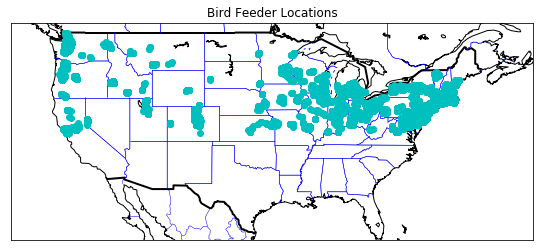
\includegraphics[width=1.0\textwidth]{figures/bf_locations_USmap.png}
\caption{The cyan colored points on the United States map represents all of the actual bird feeders used in this study. As discussed earlier, all the feeder locations are above the 38 degree latitude boundary. This avoids all observations from locations that may have mild winters. For example, birds in southern California and Texas are going to experience warmer winters than the birds in New York or Michigan simply due to geographic location. Since one of the goals of this project is to explore the reactions of bird species to cold temperatures, it is advantageous to only include geographic areas which experience relatively cold winters.}
\end{figure}

\section{Linear-mixed Effect Models}

Once the data sets were constructed, the next challenge was to pick a valid and useful model. Here Professor Francis was of great help as he had the most expertise in which data model was applicable. The linear-mixed effect model was chosen as it allows us to observe relationships among multiple variables and grouping factors in the data set, more on this later. The linear-mixed effect model is a few degrees higher in complexity than the simple linear model, so it is worthwhile to cover the basics of these models before continuing any further.     
 
Lets start at the beginning with the basic linear model. A hypothetical relationship of interest can be represented as this formula:

\[ y \sim x \]

This formula reads as ``y as a function of x'' or it can also be referred to as ``y predicted by x''. For this paper, the two terms are considered equivalent and is used interchangeably. The y in this case is considered a dependent variable. The variables to the right of the $\sim$ symbol are referred to as the predictor or independent variables. In the formula above the only predictor variable is the x, since it is a simple linear relationship. The predictor variables can also be referred to as fixed effects, but this is not relevant yet.

In real world studies, no relationship is just defined by 1 effect as with y being completely determined by x. This is far too deterministic. Other effects at play must be accounted for in the model. There may be many ``random factors'' at play. To account for this lets add another term to the formula:

\[ y \sim x + \epsilon\]

This new additive factor, $\epsilon$, it accounts for all of the random error. This term stands for everything that effects y that is not x. In other words, from our perspective the $\epsilon$ accounts for all the effects that are uncontrollable by us. This formula is the schematic depiction of the model that would be built using a statistical tool. Now that the simple formula is defined lets take steps towards building the linear-mixed model formula.

First lets add another fixed effect, say ``a'', resulting in this formula:

\[ y \sim x + a + \epsilon\]

It is important to note that ``a'' is added with plus sign, indicating an additive relationship. An additive effect is such that the affect of a on y is not dependent on the affect of x on y. The variables are independent from each other in this sense. This brings up one of the important assumptions of the linear model. The linear model assumes that all of the predictor variables are independent from each other. Logically, this makes sense as if there are 2 or more similarly effecting predictor variables, then it become difficult to identify which predictor is playing the larger role~\cite{RMixedEffect:online}.

Now it is time to introduce the random effects, and in order to illustrate this concept lets make the example more concrete and relevant. Though the formula below appears similar to the actual study, it is completely hypothetical and only for explanatory purposes. Lets say that we wanted to explore the relationship between the number of birds seen at the feeders, mean temperature and precipitation. Also assume that there are different bird species in the data set, this is important for the random effects. The formula looks like this now:

\[ Nseen \sim temp + precip + \epsilon\]

Recall that one of the major assumptions for using the linear model is the independence of the predictors, but multiple responses from the same bird species violates this assumption. This is because individuals from the same species are going to behave similarly. The similarity within species is going to be an idiosyncratic factor that affects all responses from the same species. If this is unaccounted for then the responses will be rendered inter-dependent and not independent. 

These species specific differences are accounted for in the linear model with the assumption of random intercepts for each species. Essentially this means that each bird species is assigned a different intercept value when the groupings are accounted for, but the line estimates for the groups will have the same slope value as the overall line model for the fixed effects~\cite{RandomInt:online}. These intercept estimations are calculated for each species groupings. These intercepts are the points where the line estimates for each of the species crosses the y-axis. In other words, when temp and precip have the values of 0 for their linear models.

To account for the grouping of species, a random effect is added to the formula:

\[ Nseen \sim temp + precip + (1|species) + \epsilon\]

The bird species term appears to be complicated, but that is only due to the syntax. This syntax mirrors the R programming language, which was used to construct the actual models for this study. This is covered in great detail in the later sections. The ``species'' term translates to ``assume a different intercept for each bird species''. The ``1'' stands for the intercept~\cite{RMixedEffect:online}. The formula above represents a linear-mixed effect model 

Now perhaps it becomes more clear why this model is named ``mixed''. In the earlier models only the fixed effects, or predictor variables, were taken into account. And then there was a generic error term that added. Now essentially there is more structure to that epsilon error term through the addition of a random effect. However, the $\epsilon$ is still present in the formula above because there are differences present within the species groups. The epsilon errors were calculated for all of our actual models, but the values were not used in the analysis. Instead only the defined random effects were used in the final analysis.

\section{R Programming Language and Linear Modeling}

\definecolor{codegreen}{rgb}{0,0.6,0}
\definecolor{codegray}{rgb}{0.5,0.5,0.5}
\definecolor{codepurple}{rgb}{0.58,0,0.82}
\definecolor{backcolour}{rgb}{0.95,0.95,0.92}

\lstdefinestyle{mystyle}{
    backgroundcolor=\color{backcolour},   
    commentstyle=\color{codegreen},
    keywordstyle=\color{magenta},
    numberstyle=\tiny\color{codegray},
    stringstyle=\color{codepurple},
    basicstyle=\footnotesize,
    breakatwhitespace=false,         
    breaklines=true,                 
    captionpos=b,                    
    keepspaces=true,                 
    numbers=left,                    
    numbersep=5pt,                  
    showspaces=false,                
    showstringspaces=false,
    showtabs=false,                  
    tabsize=2
}

\lstset{style=mystyle}

For this project all of the data modeling was done through the use of the R programming language~\cite{RManual}. This is because R has a robust set of packages that provides powerful statistical analysis. Additionally, our biology expert, Professor Francis, is well versed in the use of R for biological studies.

The formulas presented in the above sections are just schematic descriptions. The lme4 package of R allows us to actually build the linear models and analyze the relationships~\cite{lme4Usage}. The relationships are analyzed through the model summary, which is presented through a table. It is best to illustrate this with the continued example of the hypothetical bird species study formula:

\[ Nseen \sim temp + precip + (1|species) + \epsilon\]

The R code for constructing and summarizing the model is presented below. Notice the lack of the $\epsilon$, or the random error variable. The lmer method automatically accounts for the random error, without the explicit declaration in the parameters. However, the random error values are not of particular importance in this study and are ignored for the remainder of the analysis. 

\begin{lstlisting}[language=R]
model <- lmer(NSeen ~ temp + precip + (1|species))
summary(model)
\end{lstlisting}

The output of the ``summary'' method is presented in Tables 3.2 and 3.3. As a reminder no actual model was built as there is no data set, the tables are only for explanatory purposes. Lets first focus on Table 3.2. This table shows all of the fixed effects and their relationships to the abundance of the bird species. The ``Intercept'' row covers the y intercept of the estimated line, the standard error and the t value. The intercept is estimated through the line models when all of the predictor variables are 0. Recall, the predictor variables are ``temp'' and ``precip''. The intercept estimate is not applicable to this study. The ``Estimate'' column presents the slope estimates for each of the fixed effects. For example, there is a positive slope estimate of 2.02 associated with temp, indicating that as the temp value increased so did the Nseen value. ``SE'' is the column representing the standard error and finally there is the ``t value'' column. The standard error is for the slope estimate value and is used to calculate the t value. The t value is very crucial for this study and is covered in great detail in the Significance and t value section.

The other table that is included with model summary is the Random Effects, represented by Table 3.3. It is important to note the variance strengths, shown in the ``Variance'' column, among the different random effects. In this case we only have one random effect, but nonetheless it has caused some variance among the data. This indicates that it was useful to account for this in the data model. The other column is the ``Std. Dev.''. This is measure of how much variability in the dependent measure there is due to bird species~\cite{RMixedEffect:online}. For this study, a simple check was done with every constructed model to make sure the Random Effects table showed variances for the variables chosen. This is covered in more detail in the Data Models for this Study section.   


% Please add the following required packages to your document preamble:
% \usepackage{longtable}
% Note: It may be necessary to compile the document several times to get a multi-page table to line up properly
\begin{longtable}[c]{|l|l|l|l|}
\caption{Model Summary for the hypothetical situation of modeling bird abundance, temperature and precipitation.}
\label{my-label}\\
\hline
Fixed Effects     & Estimate  & SE       & t value \\ \hline
\endhead
%
Intercept         & 7.09  & 4.8 & 1.477  \\ \hline
temp              & 2.02 & 1.6 & 1.263 \\ \hline
precip            & -4.32  & 2.47 & -1.749   \\ \hline
\end{longtable}

% Please add the following required packages to your document preamble:
% \usepackage{longtable}
% Note: It may be necessary to compile the document several times to get a multi-page table to line up properly
\begin{longtable}[c]{|l|l|l|l|}
\caption{Random effects for the hypothetical situation of modeling bird abundance, temperature and precipitation.}
\label{my-label}\\
\hline
Groups               & Name      & Variance & Std.Dev. \\ \hline
\endhead
%
species              & Intercept & 2.24019  & 1.49009  \\ \hline

\end{longtable}

\section{Significance and t value}

The t value is very important for the analysis portion of this study. This value is calculated by dividing the ``Estimate'' by the ``SE''. The resulting value is a measure of the fixed effect strength as well as the  significance of the relationship presented by the model. The t value is a more reliable measure of the effect strength than just the slope magnitude because it takes into account the standard error. The t value is a major component in comparing how different climatic factors affect the bird abundance at the feeders and at what strengths.

The second importance of the t value comes in the form of significance. We used t values as a proxy for assessing the strength of the effect of predictor variables because the lme4 package does not calculate p-values. In essence, when the magnitude of t is greater than or equal to 2, the standard error of the effect size will be less than 1/2 the absolute value of the effect. In other words, this means the 95 percent confidence interval would never overlap zero with t greater than 2.

The confidence intervals were calculated for each of the models constructed using the R method confint. This method takes the constructed model as a parameter and returns the lower and upper bounds of the confidence interval. The effects were considered significant, if this range did not overlap zero. As explained in the previous paragraph, this non-overlap of zero is obtained if the absolute t value is greater than or equal to 2. As such, from this point on the significance of the effect is only going to be quantified by the t value.

\section{Assumptions}

As with any other model, the linear-mixed model comes with assumptions that have to be satisfied in order for the linear model to be meaningful~\cite{RLinear:online}. To check that the assumptions are satisfied, a simple test can be performed with the residual values. A residual value is the difference between the observed dependent variable and the predicted value from the line estimate~\cite{Residuals:online}. If the histogram of the residuals follows an approximately normal curve then one can assume the assumptions are met as the distance of the data points from the line estimate follow a roughly normal curve when plotted~\cite{LinRegress:online, LinearAssump:online}.

The residual histograms were inspected individually by eye, as quantitative methods in R were not advanced enough to detect approximate normal distributions. Too many of the rough normal distributions were rejected by these methods, thus it was decided to check every histogram by eye. In addition to the histograms, Q-Q plots for the residual values were also created and inspected. A Q-Q plot is a scatterplot created by plotting 2 sets of quantiles, or percentiles, against one another~\cite{QQPlots:online}. If both sets of quantities came from the same distribution, then we should see the points forming a line~\cite{QQPlots:online}. For this study the residual values need to follow an approximately normal distribution, as such the residual quantiles are plotted against the normal distribution quantiles. If the residuals follow an approximately normal distribution then the points should roughly follow a line. These specific Q-Q plots are referred to as Q-Q normal plots. One histogram and one Q-Q normal plot were constructed and inspected for each of the data models built. This process is covered in detail in the next section.


\section{Data Models for this Study}

\definecolor{codegreen}{rgb}{0,0.6,0}
\definecolor{codegray}{rgb}{0.5,0.5,0.5}
\definecolor{codepurple}{rgb}{0.58,0,0.82}
\definecolor{backcolour}{rgb}{0.95,0.95,0.92}

\lstdefinestyle{mystyle}{
    backgroundcolor=\color{backcolour},   
    commentstyle=\color{codegreen},
    keywordstyle=\color{magenta},
    numberstyle=\tiny\color{codegray},
    stringstyle=\color{codepurple},
    basicstyle=\footnotesize,
    breakatwhitespace=false,         
    breaklines=true,                 
    captionpos=b,                    
    keepspaces=true,                 
    numbers=left,                    
    numbersep=5pt,                  
    showspaces=false,                
    showstringspaces=false,
    showtabs=false,                  
    tabsize=2
}

\lstset{style=mystyle}

The R code for modeling the actual constructed data set is below. Notice that the syntax is very similar to the formulas discussed before. Besides the 3 flags at the end of the parameters, the formula schema is almost identical in format to the previous schematics.    

\begin{lstlisting}[language=R]
model <- lmer(log(NSeen) ~ temp_anomalies + scale(wspeed_kmph) 
               + precip_anomalies + (1|EFFORT_HRS_ATLEAST) + (1|LOC_ID) 
               + (1|NHalfDays) + (1|city), REML=F, data=dat1, 
               na.action="na.fail")
\end{lstlisting}

The linear mixed-effect model is constructed using the lmer function, with the returned data model stored in the variable model. One model was built for each of the 23 bird species, using the same R code and methods. The results of these species specific linear models are discussed in the Results section. The key components of the lmer function are the parameters, as they determine which variables to build the linear models with. 

In addition to the 23 models for each of the species, one other general model was built to encompass all of the bird species. The only difference in construction of this model is the inclusion an additional random effect (1\textbar BirdSpp), or bird species. This allows the data points to be grouped by bird species. The code for constructing the generalized linear-mixed effect model is below.

\begin{lstlisting}[language=R]
model <- lmer(log(NSeen) ~ temp_anomalies + scale(wspeed_kmph) 
               + precip_anomalies + (1|EFFORT_HRS_ATLEAST) +	(1|LOC_ID) + (1|NHalfDays) + (1|city) + (1|BirdSpp), REML=F, data=dat2, na.action="na.fail")
\end{lstlisting}

The first variable used in the method is the log(NSeen) and this is simply the the natural log of number of individuals seen of that bird species, as discussed in the Given Attributes of the Project FeederWatch Data section. This is the dependent variable in the linear models and this followed by the $\sim$ symbol~\cite{RLinearModel:online}. That symbol indicates the term ``function of'' and is followed by the independent variables to the right. These independent variables are also known as predictor variables.

One may wonder why the natural log of the number of individuals at the feeders is used in the models. In order to illustrate why the natural log of the Nseen value was used instead of just the Nseen value, it is best to walk through a concrete example. Let's focus on the data set for the species White-throated Sparrow. The histogram of the values of Nseen for this species is presented in Figure 3.3. It is very clear that there is a left skew to the distribution. This results in a non-normal distribution of the residuals, as presented in Figure 3.4. This histogram does not exhibit an approximate normal distribution, in regards to this study. This violates the major assumption of using the linear mixed-effect model, as this model assumes an approximately normal distribution of the residuals.

\begin{figure}[h]
\centering
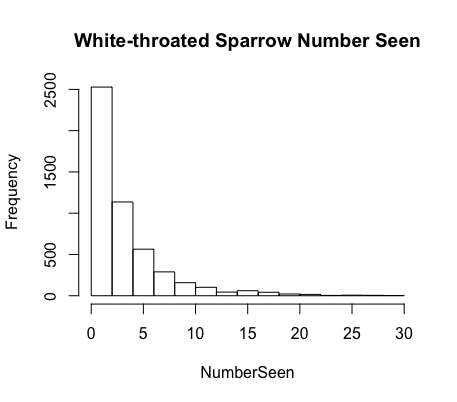
\includegraphics[width=12cm]{figures/WhiteSparrowNSeen.png}
\caption{The histogram of the Nseen values of the White-throated Sparrow.}
\end{figure}

\begin{figure}[h]
\centering
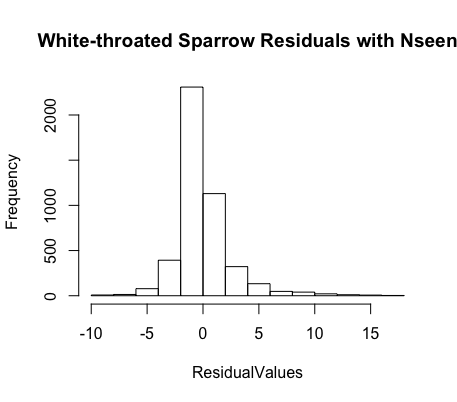
\includegraphics[width=12cm]{figures/WSResidNolog.png}
\caption{The histogram of the residual values of the linear model constructed with the Nseen values. This is for the White-throated Sparrow.}
\end{figure}


The histogram of the natural log of the Nseen is presented in Figure 3.5. There is still a left skew present, however there is a better distribution of values. The histogram of the residuals from the linear mixed-effect model with the natural log of Nseen is presented in Figure 3.6. This time the residual values follow an approximately normal distribution, thus allowing us to draw insights from the linear mixed-effect model.

\begin{figure}[h]
\centering
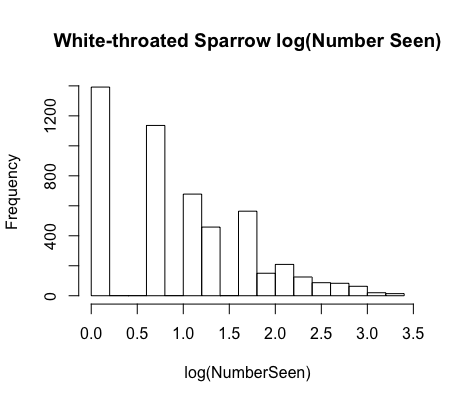
\includegraphics[width=12cm]{figures/WhiteSparrowlogNseen.png}
\caption{The histogram of the natural log of Nseen values of the White-throated Sparrow.}
\end{figure}

\begin{figure}[h]
\centering
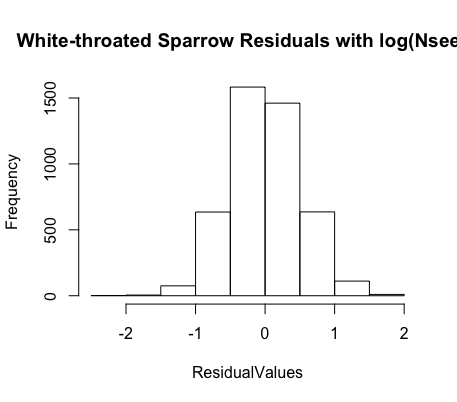
\includegraphics[width=12cm]{figures/WSResidlog.png}
\caption{The histogram of the residual values of the linear model constructed with the log(Nseen )values. This is for the White-throated Sparrow.}
\end{figure}

The predictor variables for the models of this study are temp\_anomalies, precepi\_anomalies and scale(wspeed\_kmph). These variables can also be referred to as fixed effects as they are the main focus of the analysis. Note the scale of the wind speed value is used for the models. This is because the standardized values of the wind speed allow for better comparisons against the other independent variables. Recall, the units of the wind speed values are miles per hour and the other variables, such as temperature anomalies, are just the scaled values.  

These fixed effects are added together by the addition sign to indicate they are additive properties. Recall, the addition sign indicates that the variables are to be modeled as additive effects. These effects are such that there is no dependability among the additive properties~\cite{AddProps:online}. In other words the effect of temp\_anomalies on log(NSeen) does not depend on the value of scale(wspeed\_kmph) or any of the other additive effects.

The last additive effects to cover are the random effects, otherwise known as grouping variables. The random effects allow the data models to account for the grouping of certain observations. For example, the syntax (1\textbar city) tells the method lmer to fit a linear model with a varying-intercept group effect using the variable city. In other words it specifies that all observations that have the same city attribute belong to the same group, as the weather data may have been collected from the same weather stations. As such, those tuples should not be considered independent from each other and the linear model is adjusted accordingly. Since the focus of this project is body mass and the influences of climate conditions specifically, the exact influence of city and other random effects on the log(Nseen) is ignored.    

To summarize, the grouping variables are   
(1\textbar city), (1\textbar NHalfDays), (1\textbar LOC\_ID) and (1\textbar EFFORT\_HRS\_ATLEAST). The effort of hours (NHalfDays) and number of half days (EFFORT\_HRS\_ATLEAST) are groupings based on the effort of the observer making that particular observation. This is important to take into account as different observers of PFW have varying degrees of precision in making a bird feeder observations. Additionally, one observer may submit multiple observations. Those observations need to be grouped. 

Location ID (LOC\_ID) is the location grouping. Previously the city grouping was discussed, this grouping is based on the location of the actual bird feeder. This is also important as there may be multiple observations from a single bird feeder and thus those observations should be viewed as a group. As a reminder, this location ID was already provided in the original PFW data set.

% Please add the following required packages to your document preamble:
% \usepackage{longtable}
% Note: It may be necessary to compile the document several times to get a multi-page table to line up properly
\begin{longtable}[c]{|l|l|l|l|}
\caption{Random effects for the linear-mixed model of the White-throated Sparrow.}
\label{my-label}\\
\hline
Groups               & Name      & Variance & Std.Dev. \\ \hline
\endhead
%
LOC\_ID              & Intercept & 0.24015  & 0.4901  \\ \hline
city                 & Intercept & 0.0834  & 0.2889  \\ \hline
NHalfDays            & Intercept & 0.002411   & 0.0491  \\ \hline
EFFORT\_HRS\_ATLEAST & Intercept & 0.002052  & 0.0453  \\ \hline
\end{longtable}

To clearly illustrate the effects of the grouping variables, the random effects table for the previous example of White-throated Sparrow is presented in Table 3.4. The most important attribute is the Variance, as this determines how much influence the random effect variable has on the model. The higher the variance, the stronger the effect of that variable. It is clear from the table that the LOC\_ID and the city has the most influence, while (1\textbar EFFORT\_HRS\_ATLEAST) and (1\textbar NHalfDays) has less influence, but there is influence nonetheless. For this project all of the Random Effects tables were inspected to ensure there was at least some amount of variation among the groups. A full list of the Random Effects table for each of the 23 species is presented in Appendix A.


The (1\textbar BirdSpp) term is for the generalized model as it groups observations by species name. Meaning, data points that have the same bird species name are considered non-independent from each other and thus are treated accordingly for the model. The idea here being to observe any large-scale trends that occur when considering all the species' datasets together as one large dataset. 

Finally, the last few parameters are flags and the source of the data. The REML=F flag forces the model to use the maximum likelihood for parameter estimates rather than restricted maximum likelihood (REML). The relevance of this is that if flag was the default value of REML then it may produce a non-reliable model. This is especially true when you compare models with different effects, which is true for this analysis.

The data= term sets the data source. The data source for the 23 models were the 23 data frames, one for each bird species. Data frames are a form of data representation that allows the code methods to process it. In other words, raw data of many formats are converted to data frames to be used in code functions. For the generalized model, the data source was the combined data frame which contained all of tuples from each of the 23 species. The data frames contain all of the attributes required for constructing the models. In the end, a total of 23 linear-mixed models were constructed and analyzed, one for each bird species. In addition, a general model was constructed with all of the species combined.

The na.action= ``na.fail'' flag sets the action for the method when a null value in the parameters of lmer is encountered. The ``na.fail'' ensures that the linear-mixed model object is only returned by lmer if there are no null values in the method arguments. All of the null values were removed from the constructed datasets during the preprocessing steps before the lmer method was actually called, but the flag ensures that no null values were overlooked.   

\section{Model Outputs}

The returned object from the method lmer is the constructed linear-mixed model. The R summary method is then called on this returned model. This summary method returns the slope estimates, standard errors for the slope estimates and the t value for each of the independent variables. As reminder, the t value is the slope estimate divided by the standard error value. Also recall that the independent variables for this study are the temperature anomalies, precipitation anomalies and scaled wind speeds. The full summary table for the White-throated Sparrow linear-mixed model, which includes all of the attributes for each fixed effect, is presented in Table 3.5.

% Please add the following required packages to your document preamble:
% \usepackage{longtable}
% Note: It may be necessary to compile the document several times to get a multi-page table to line up properly
\begin{longtable}[c]{|l|l|l|l|}
\caption{Model Summary for White-throated Sparrow. Recall that fixed effects is another name for independent variables.}
\label{my-label}\\
\hline
Fixed Effects     & Estimate  & SE       & t value \\ \hline
\endhead
%
Intercept         & 7.09E-01  & 4.88E-02 & 14.522  \\ \hline
Temp. Anom.       & -2.02E-02 & 1.66E-03 & -12.183 \\ \hline
scale(wind speed) & 5.18E-03  & 1.03E-02 & 0.503   \\ \hline
Precip. Anom.     & 4.32E-03  & 6.47E-03 & 0.667   \\ \hline
\end{longtable}

The slope estimate, labeled ``Estimate'', of the linear model is the effect of the climate attributes on the natural log of the number seen of the species. For example, lets just focus on the temperature anomalies. If the the slope is a negative value then more individuals of the bird species were seen at the feeders when the mean daily temperatures were lower than the average winter temperature for that year. If the slope estimate is a positive value, then as the temperature anomalies got more negative the less the individuals visit the bird feeders. In other words, as the temperature increased more individuals of the species were observed. Recall that slope magnitude is not an accurate measure of effect strength. The effect strength is measured by the t value. 

The t value is also analogous to the statistical p-value in terms of model significance, except for the fact that models must have a value of above 2 or less than -2 in order to be considered significant. With p-value, results are considered significant if the p-value is below 0.05~\cite{p-value:online}. For this project, the t value is also a measure of how strong the effect of that particular climate attribute is on the number of individuals seen at the feeders. For example, lets take the anomalies from precipitation levels. If the absolute value of the t value for this fixed effect is lower than 2, then the relationship is not significant enough to warrant insights. If the t value is above 2 then we can safely draw insights from the relationship as the effect of precipitation is strong enough~\cite{t-value:online}. 

The magnitude of the absolute value of the t value is also significant, as the greater the value the stronger the effect~\cite{t-value-interp:online}. For example, lets say one species has a t value of 2.5 while another bird species has a t value of 4.5. The second species is more effected by the anomalies in precipitation than the first species.  

\section{Residual Values}

In order to use the linear-models for analysis, the main assumption is that the residual values must have an approximately normal distribution. A histogram for each of the 23 bird species' data models and the generalized data model was created and inspected to ensure normal distribution. This process was done through visual inspection. This conclusion was reached after talks with Professor Francis, who has years of experience modeling biological data.

Two examples of what we determined to be approximate normal distributions are presented in Figures 3.7 and 3.8. These are the residual values for the bird species White-throated Sparrow and Northern Cardinal, respectively. Finally, Figures 3.9 and 3.10 present the histograms of the residuals that we deemed not approximately normal. They are from the species Hairy Woodpecker and Red-bellied Woodpecker, respectively. 

\begin{figure}[h]
\centering
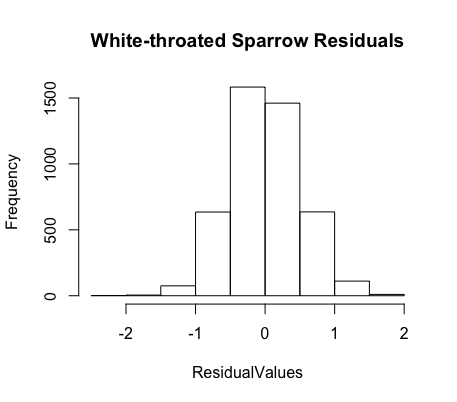
\includegraphics[width=10cm]{figures/WhiteSpResid.png}
\caption{Residual values from the White-throated Sparrow data.}
\end{figure}

\begin{figure}[h]
\centering
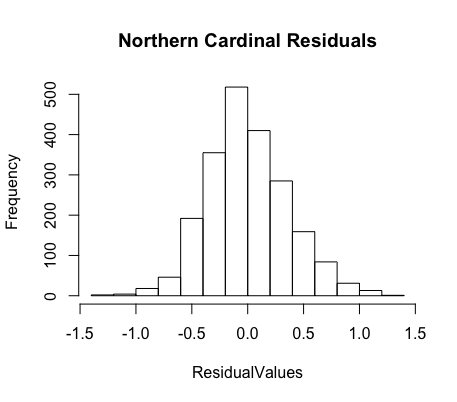
\includegraphics[width=10cm]{figures/NorthCardResid.png}
\caption{Residual values from the Northern Cardinal data.}
\end{figure}

\begin{figure}[h]
\centering
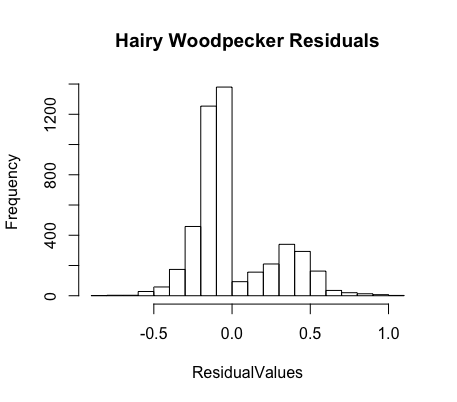
\includegraphics[width=10cm]{figures/HairyWoodResid.png}
\caption{Residual values from the Hairy Woodpecker data.}
\end{figure}

\begin{figure}[h]
\centering
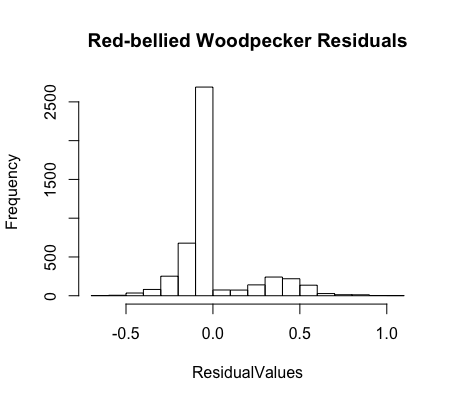
\includegraphics[width=10cm]{figures/redbwoodResid.png}
\caption{Residual values from the Red-bellied Woodpecker data.}
\end{figure}

Lastly, Q-Q normal plots for the residual values were also created and inspected to ensure the approximate normal distributions. For these scatter plots, if the points approximately form a line, then one can assume the residual values follow a rough normal distribution. An example of a Q-Q normal plot representing an approximately normal distribution is presented in Figure 3.11. This plot is for the White-throated Sparrow. And finally, a Q-Q normal plot representing a non-normal distribution is presented in Figure 3.12. This plot is for the Hairy Woodpecker.

\begin{figure}[h]
\centering
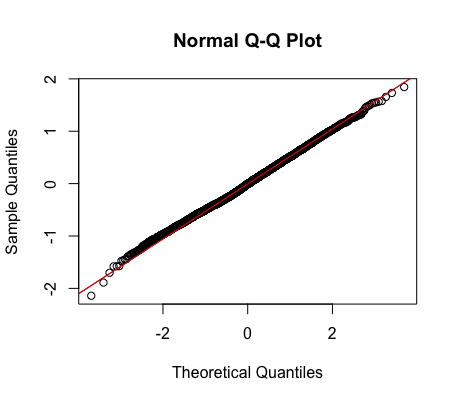
\includegraphics[width=10cm]{figures/whtspa_qqplot.png}
\caption{Residual values from the White-throated Sparrow data. Observe how the majority of the points follow the red line.}
\end{figure}

\begin{figure}[h]
\centering
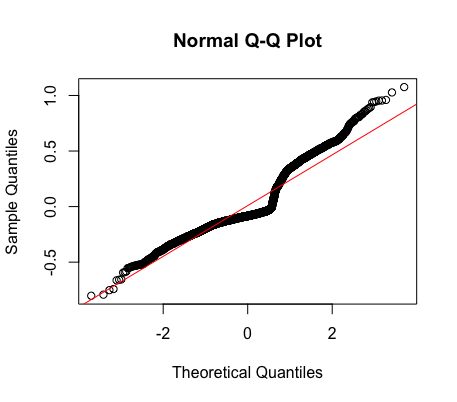
\includegraphics[width=10cm]{figures/haiwoo_qqplot.png}
\caption{Residual values from the Hairy Woodpecker data. Observe the major deviations from the red line.}
\end{figure}
